\documentclass[tikz]{standalone}
\usetikzlibrary{calc,patterns,angles,quotes}
\usepackage{pgfplots}
\pgfplotsset{compat=newest}

\pagestyle{empty}

\begin{document}
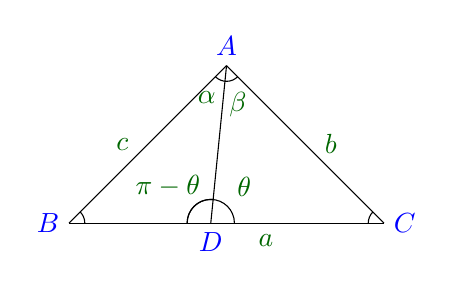
\begin{tikzpicture}
  \coordinate [label={[blue]above:$A$}] (A) at (0, 2);
  \coordinate [label={[blue]right:$C$}] (C) at (2, 0);
  \coordinate [label={[blue]left:$B$}] (B) at (-2, 0);
  \coordinate [label={[blue]below:$D$}] (D) at (-0.2, 0);
  \draw (B) -- (C);
  \draw (A) -- (B);
  \draw (C) -- (A);
  \draw (D) -- (A);
  \node[label={[black!60!green]left:$c$}] at ( $ (A)!0.5!(B) $ ) () {};
  \node[label={[black!60!green]below, xshift=0.5cm, yshift=0.1cm:$a$}] at ( $ (C)!0.5!(B) $ ) () {};
  \node[label={[black!60!green]right:$b$}] at ( $ (C)!0.5!(A) $ ) () {};
  \draw pic [draw, angle radius=0.2cm] {angle=B--A--C};
  \draw pic [draw, angle radius=0.2cm] {angle=C--B--A};
  \draw pic [draw, angle radius=0.2cm] {angle=A--C--B};
  \draw pic [draw, angle radius=0.3cm] {angle=A--D--B};
  \draw pic [draw, angle radius=0.3cm] {angle=C--D--B};
  \coordinate [label={[label distance=0.3cm, black!60!green]below left, xshift=0.2cm:$\alpha$}] (A1) at (0, 2);
  \coordinate [label={[label distance=0.3cm, black!60!green]below right, xshift=-0.3cm:$\beta$}] (A1) at (0, 2);
  \coordinate [label={[label distance=0.3cm, black!60!green]above right:$\theta$}] (D1) at (-0.2, 0);
  \coordinate [label={[label distance=0.3cm, black!60!green]above left, xshift=0.2cm:$\pi-\theta$}] (D1) at (-0.2, 0);
\end{tikzpicture}
\end{document}
